\documentclass[12pt]{article}

\usepackage{sbc-template}
\usepackage{graphicx,url}
\usepackage[utf8]{inputenc}
\usepackage[brazil]{babel}  

     
\sloppy

\title{Modelagem Preditiva de Manchas Criminais: Análise Espaço-Temporal de Roubos na Região Metropolitana de São Paulo}

\author{Aaron F. do A. M. da Silva\inst{1}, Marcos M. da Silva Filho\inst{2}, Pedro H. S. Matos\inst{3}}


\address{Escola de Artes, Ciências e Humanidades -- Universidade de São Paulo (USP)
  \email{aaronferrazamaral@usp.br, marcos\_filho@usp.br, pedrom07@usp.br}
}

\raggedbottom
\begin{document} 

\maketitle
     
\begin{resumo} 
  O enfrentamento da criminalidade urbana exige abordagens analíticas avançadas para o planejamento estratégico em segurança pública. Este projeto propõe o desenvolvimento de um modelo preditivo baseado em aprendizado de máquina para mapear áreas de risco de roubos na Região Metropolitana de São Paulo. Utilizando dados da Secretaria de Segurança Pública do Estado de São Paulo (2022 a 2026), a metodologia foca na segmentação por tipologias penais e na aplicação de uma arquitetura \textit{ensemble}. O algoritmo Random Forest servirá como linha de base para comparação com XGBoost e LightGBM. Os resultados preditivos serão integrados a uma interface de geovisualização por mapas preditivos de risco, superando as limitações dos modelos tradicionais de "caixa-preta" e fornecendo uma ferramenta interpretável para auxiliar na alocação de recursos policiais.
\end{resumo}


\vspace{0.5cm}


\section{Introdução}
A dinâmica da criminalidade urbana, particularmente no que tange aos crimes contra o patrimônio, representa um dos desafios mais complexos para a gestão da segurança pública em áreas de alta densidade demográfica. Na Região Metropolitana de São Paulo (RMSP), a confluência de fatores socioespaciais, vulnerabilidades estruturais e intensa mobilidade urbana cria um cenário propício para a ocorrência sistemática de roubos, exigindo das autoridades estratégias de prevenção cada vez mais sofisticadas. Historicamente, o enfrentamento dessas ocorrências tem se fundamentado em abordagens táticas reativas, baseadas na alocação de recursos apenas após a consumação e o registro do delito. Contudo, o avanço das técnicas de Ciência de Dados e a crescente disponibilidade de bases governamentais abertas têm impulsionado uma necessária mudança de paradigma. A aplicação de algoritmos de aprendizado de máquina (\textit{Machine Learning}) sobre grandes volumes de dados criminais permite a transição para um modelo de policiamento preditivo, focado na antecipação do risco e na identificação de padrões espaço-temporais que caracterizam a formação das chamadas manchas criminais.

Apesar dos avanços proporcionados pelo uso computacional na segurança pública, o mapeamento do estado da arte revela lacunas metodológicas significativas na modelagem deste fenômeno. Trabalhos correlatos recentes têm explorado correlações entre a criminalidade e indicadores de vulnerabilidade socioeconômica, além de compararem o desempenho de diferentes algoritmos preditivos. No entanto, constata-se uma escassez de abordagens que combinem, de forma integrada, a predição espacial avançada com a categorização minuciosa dos subtipos de delitos. Ao tratar o crime de roubo como uma classe homogênea e única, perdem-se as especificidades comportamentais e geográficas inerentes a modalidades distintas, como o roubo de veículos em contraste com o roubo de celulares. Adicionalmente, abordagens baseadas exclusivamente em algoritmos de "caixa-preta" esbarram na falta de explicabilidade, um requisito fundamental para a adoção de ferramentas tecnológicas no planejamento tático de segurança.

\begin{figure}[ht]
\centering
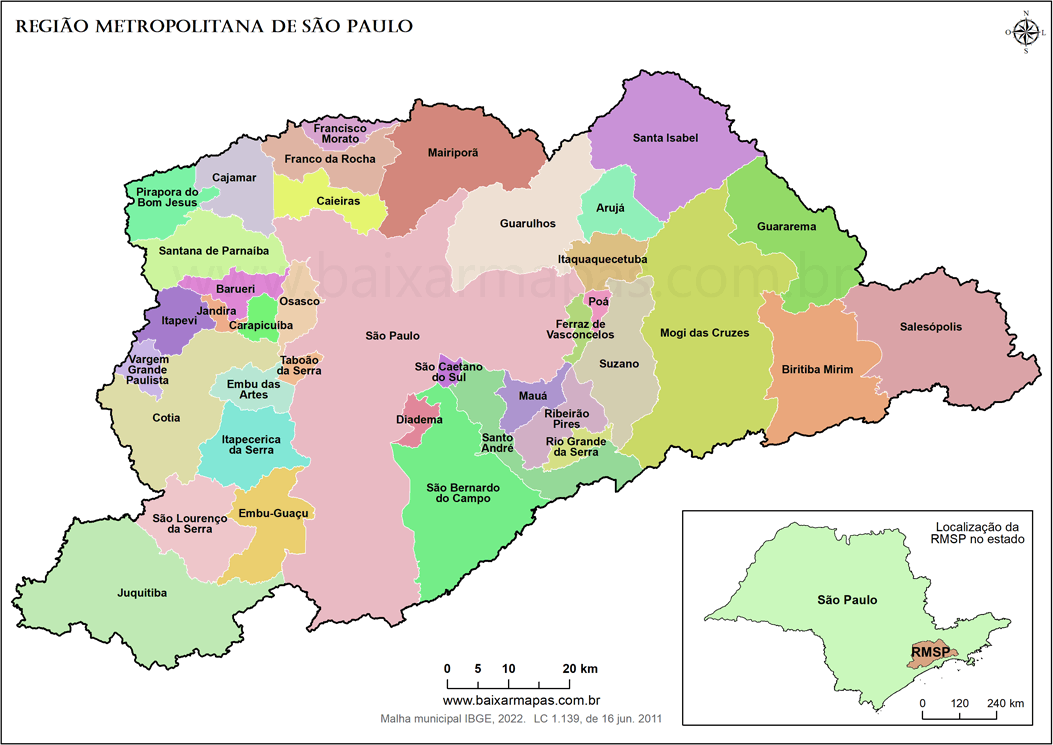
\includegraphics[width=.7\textwidth]{mapa-regiao-metropolitana-sao-paulo-municipios.png}
\caption{Região Metropolitana de São Paulo \cite{baixarmapas2026}}
\label{fig:mapa_rmsp}
\end{figure}

Para mitigar essas limitações, este artigo tem como objetivo principal propor um modelo preditivo para a identificação e o mapeamento de áreas de risco de roubos na RMSP. Diferente de abordagens mais restritas, a pesquisa propõe a decomposição do problema por tipologias penais, utilizando dados da Secretaria de Segurança Pública do Estado de São Paulo (SSP-SP). A intenção é construir índices de risco específicos para cada natureza operacional, fornecendo não apenas predições estatísticas de alta precisão, mas também uma interface visual interpretável por meio de mapas preditivos de risco.

Dessa forma, a principal contribuição deste trabalho é fornecer uma solução analítica focada em explicabilidade e segmentação espacial, subsidiando a tomada de decisão estratégica e a alocação mais eficiente de recursos pelas forças de segurança pública do Estado de São Paulo.  



\vspace{1.2cm}

\section{Trabalhos Relacionados}
Com o intuito de mapear o estado da arte e identificar as abordagens vigentes sobre a temática, realizou-se um levantamento bibliográfico que resultou na seleção de três trabalhos diretamente correlacionados ao tema desta pesquisa.

O primeiro estudo selecionado \cite{couto2024identificaccao} investiga os padrões comportamentais e espaciais associados ao roubo de celulares no Rio Grande do Sul. Empregando a técnica de agrupamento não supervisionado K-means integrada a variáveis geográficas e sociodemográficas. O autor buscou correlacionar a incidência do crime às vulnerabilidades socioeconômicas locais. Os resultados evidenciaram que tanto as vítimas quanto os autores dos delitos concentram-se majoritariamente em bairros periféricos de Porto Alegre, caracterizados por baixos índices de desenvolvimento humano (IDH) e menor poder aquisitivo.

Paralelamente, \cite{de2025previsao} avaliaram o desempenho comparativo entre Árvores de Decisão e Redes Neurais na predição de roubos de veículos no município do Rio de Janeiro. Embora os resultados tenham demonstrado a superioridade preditiva das Redes Neurais, os autores ressaltam uma limitação crítica: a falta de explicabilidade associada à sua natureza de 'caixa-preta', aspecto essencial para tomada de decisões estratégicas em segurança pública.

Por fim, o estudo conduzido por \cite{fernandes2025aplicaccao} investigou os determinantes socioeconômicos e estruturais associados à criminalidade nos municípios do estado de São Paulo. Utilizando o algoritmo XGBoost, o modelo ajustado alcançou um coeficiente de determinação que explicou 98,5\% da variabilidade dos dados. A interpretação dos resultados via valores SHAP (SHapley Additive exPlanations) confirmou que a vulnerabilidade socioeconômica atua como um dos principais fatores impulsionadores das elevadas taxas de criminalidade regional.

A partir do mapeamento da literatura, constata-se a ausência de abordagens que combinem a visualização espacial por meio de mapas preditivos de risco com a categorização detalhada dos subtipos de roubo. Visando preencher essa lacuna, a presente pesquisa diferencia-se dos estudos anteriores sob três aspectos centrais: no recorte geográfico focado na Região Metropolitana de São Paulo, na delimitação temporal (compreendendo o período de 2022 ao primeiro semestre de 2026) e no escopo dos dados, direcionado exclusivamente aos roubos e suas especificidades. Adicionalmente, além da avaliação de outros algoritmos de aprendizado de máquina, será incorporado o XGBoost, em alinhamento com os bons resultados reportados por \cite{fernandes2025aplicaccao}.

\vspace{1.2cm}

\section{Metodologia}
Para o desenvolvimento de um modelo preditivo para identificação de áreas com risco a roubos, será utilizada a base de dados criminais de 2022 até 2026 da Secretaria de Segurança Pública do Estado de São Paulo (SSP-SP)\footnote{\url{https://www.ssp.sp.gov.br/estatistica/consultas} Acesso em: 22/08/2026}. Serão coletadas as fontes e unificadas em um único arquivo, mantendo, posteriormente, somente registros relacionados a roubos pertencentes às cidades da Região Metropolitana de São Paulo.

Com a base unificada, será feita uma Análise Exploratória dos Dados para entender a natureza do problema, identificar ruídos e padronizar de acordo com as necessidades do algoritmo, além de retirar as quantidades de ocorrência por crime, localização, mês e ano para possibilitar o cálculo do risco.

A modelagem preditiva adotará uma abordagem de \textit{ensemble}. O modelo será estruturado a partir da decomposição do problema por tipologias de roubos (e.g., roubo de veículos, roubo de celular), treinando-se estimadores específicos para cada categoria penal. As predições individuais de risco serão posteriormente integradas por meio de uma função de agregação, gerando um índice consolidado de risco a roubo para uma determinada unidade espaço-temporal.

Para as etapas de treinamento e validação do modelo, será utilizada a série temporal correspondente ao período do primeiro semestre de 2022 ao primeiro semestre de 2025. O intervalo remanescente, englobando do segundo semestre de 2025 ao primeiro semestre de 2026, será reservado para a etapa de teste. A adoção desta partição temporal justifica-se pela limitação da base de 2026, que contém dados restritos ao primeiro semestre, e pela necessidade de assegurar que ambos os conjuntos contemplem a sazonalidade completa dos ciclos anuais da criminalidade, evitando viés no processo de avaliação do algoritmo.

Adota-se o algoritmo Random Forest como modelo de referência, estabelecendo-se uma análise comparativa com os algoritmos XGBoost e LightGBM, os quais representam o estado da arte para a modelagem de dados tabulares. O ajuste de hiperparâmetros e a otimização dos estimadores serão conduzidos na etapa de validação por meio de validação cruzada temporal, preservando a cronologia das ocorrências. A partir dessa etapa, a configuração de melhor desempenho será selecionada e submetida à avaliação final no conjunto de teste, permitindo mensurar a capacidade de generalização e eficácia preditiva do modelo proposto.

Após a consolidação e validação do modelo preditivo, as inferências de risco serão integradas a uma interface de geovisualização fundamentada em mapas preditivos de risco para a Região Metropolitana de São Paulo. A solução permitirá a representação cartográfica da intensidade do risco de roubo de forma espacialmente desagregada, possibilitando tanto a análise do indicador de risco global quanto a filtragem por tipologias criminais específicas (e.g., roubo de veículos, celulares). Essa abordagem visual visa subsidiar a identificação precisa de manchas criminais e o diagnóstico de padrões espaciais, fornecendo suporte analítico para a tomada de decisão e o planejamento estratégico em segurança pública.

\vspace{1.2cm}
\section{Resultados Parciais}
Primeiramente, foi necessário algumas decisões para obter a base tratada. Dentre elas, foi preencher a informação da cidade da ocorrência com a cidade do registro, pois cerca de 10%

\clearpage
\section{Cronograma}
O planejamento da pesquisa foi estruturado de acordo com as datas da disciplina de Resolução de Problemas II com a docente Profa. Dra. Karina Valdivia Delgado. Adotamos desde a entrega do plano de pesquisa até a conclusão e apresentação do projeto.

\begin{table}[htpb]
    \centering
    \caption{Cronograma de execução e marcos de entrega da pesquisa.}
    \label{tab:cronograma}
    \vspace{0.2cm} % Espaço entre o título e a tabela
    \begin{tabular}{p{3.5cm} p{11cm}}
        \hline
        \textbf{Período / Data} & \textbf{Atividade ou Marco de Entrega} \\
        \hline
        26/08 & \textbf{Entrega do Plano de Trabalho:} Definição formal da concepção do artigo científico. \\
        
        02/09 a 16/10 & \textbf{Desenvolvimento do Trabalho:} Tratamento da base de dados da SSP-SP, Análise Exploratória de Dados, especificações dos algoritmos, criação e treinamento do modelo. \\
        
        21/10 & \textbf{Entrega do Relatório Parcial e Vídeo:} Documentação dos resultados preliminares do modelo, identificação de lacunas a serem corrigidas, vídeo sobre estado atual do projeto. \\
        
        23/10 a 13/11 & \textbf{Finalização do Trabalho:} Validação final do modelo \textit{ensemble} (Random Forest, XGBoost e LightGBM), geração dos mapas preditivos de risco e relatório conclusivo do artigo. \\
        
        18/11 & \textbf{Entrega do Relatório Final:} Submissão do documento científico consolidado. \\
        
        25/11, 27/11, \newline 02/12 e 04/12 & \textbf{Apresentação do Trabalho:} Compartilhamento da nossa proposta e resultados obtidos perante a turma da disciplina. \\
        \hline
    \end{tabular}
\end{table}


\vspace{1.2cm}

\bibliographystyle{plain}
\bibliography{referencias}


\end{document}



